% !TeX program = pdflatex
% =============================================================================
% Arbeitsblatt 5: Wechselwirkung
% UZH Praktikum I -- Sara Romer Urban, Kantonsschule im Lee, HS2026
% Klasse: 2e (16.09.2026)
%
% Folgt der in lernziele.md festgelegten Aufteilung ("Aufteilung Arbeitsblatt/
% Aufgabenblatt und Zeitbudget"): Einstieg (Werkstatt-Kraft-Rueckblick, formales
% Wechselwirkungsgesetz, Abgrenzung zum Kraeftegleichgewicht, LZ1) -> Aktivierung
% (Skateboard-Experiment, alle drei Varianten als Predict-Observe-Explain,
% Bilder/Skateboard1/3/4, LZ4) -> Zeichenaufgabe (Federwaage-Kette,
% Bilder/federwaage.png + zwei Loesungsbilder, LZ2 erster Teil) -> Experiment
% (Federwaage zwischen zwei 200g-Massen, Bilder/Federwaage_zwei_massen.jpg, LZ3)
% -> Vertiefung (LKW-PKW-Predict, Bilder/LKW_vs_PKW.png, + PhysikLibre-
% Eisflaeche-Beispiel, LZ4 Fortsetzung) -> Vertiefung (Magnetwagen als
% Gedankenexperiment OHNE Observe-Schritt, da der Wagen nicht real existiert
% und im Unterricht nicht gezeigt werden kann, Bilder/magnetauto.png, +
% Lok auf drehbarem Rad als echtes, im Unterricht zeigbares
% Predict-Observe-Explain-Experiment, Bilder/lok_auf_rad.jpg, LZ5) ->
% Beispiele (Rakete, Bilder/Rakete.jpg, als Kernbeispiel Rueckstossprinzip,
% LZ6, Auswahl) -> Abschluss (eigene Alltagssituation, im Plenum
% besprochen, LZ7).
%
% Das zweite in lernziele.md fuer diese Phase vorgeschlagene Kernbeispiel,
% Eisflaeche, wird hier bewusst NICHT als eigene Aufgabe wiederholt: Es wurde
% bereits in der Vertiefung zuvor (LZ4, PhysikLibre 4.2.8 neben LKW-PKW)
% inhaltlich behandelt und ist an dieser Stelle nur noch als kurzer
% Querverweis in der (fuer SuS unsichtbaren) Loesung der LKW-PKW-Aufgabe
% eingebaut (Redundanzvermeidung, siehe redundanz-tiefe-reviewer). Die
% Rueckstossprinzip-Aufgabe (Rakete) verweist deshalb NICHT mehr auf ein
% "Eisflaechenbeispiel von vorhin" zurueck -- aus Sicht der SuS gibt es
% keines, da der Querverweis nur im Lehrpersonen-Loesungstext steht.
%
% Praktikum I: Sie-Form, keine farbigen Boxen ausser Formel-/Hinweis-/Antwortbox,
% Textmenge knapp (Sara Romers Feedback ab Kondensatoren). Boxen-Definitionen aus
% arbeitsblatt4-normalkraft.tex uebernommen.
%
% Quellen: lernziele.md (dieser Ordner).
% =============================================================================
\documentclass[addpoints,11pt,a4paper]{exam}

\usepackage[T1]{fontenc}
\usepackage[utf8]{inputenc}
\usepackage[ngerman]{babel}
\usepackage{lmodern}
\usepackage[a4paper,margin=2.2cm,headheight=14pt]{geometry}
\usepackage{amsmath}
\usepackage{siunitx}
% Hausstil: zusammengesetzte Einheiten immer als echter Bruch (\frac), nicht
% als Inline-Schraegstrich oder \tfrac -- gilt global fuer jedes \si/\SI.
\sisetup{per-mode=fraction,fraction-command=\frac}
\usepackage{array,booktabs,tabularx,multirow}
\usepackage{enumitem}
\usepackage{xcolor}
\usepackage{colortbl}
\usepackage{tikz}
\usepackage{physics}
\usepackage[most]{tcolorbox}
\usepackage{lastpage}
\usepackage{graphicx}
\usepackage{hyperref}

\usetikzlibrary{arrows.meta,calc,angles,quotes,decorations.pathmorphing}

\usepackage{setspace}
\usepackage{needspace}
\setlength{\parindent}{0pt}
\setlength{\parskip}{0.6em}
\setstretch{1.08}
\setlist[itemize]{itemsep=0.4em}

% -----------------------------
% Farben (Corporate-Farbschema Physik KFR)
% -----------------------------
\definecolor{titleblue}{HTML}{183A6B}
\definecolor{accentblue}{HTML}{2E6F9E}
\definecolor{lightblue}{HTML}{EAF4FB}
\definecolor{lightgray}{HTML}{F4F6F8}
\definecolor{darkgray}{HTML}{4A4A4A}
\definecolor{accentorange}{HTML}{D9720C}
\definecolor{accentpurple}{HTML}{7B2D8E}
% Hinweisbox: Orange (accentorange), fuer wichtige Klarstellungen.
\definecolor{lightorange}{HTML}{FCEEE0}
% Formelbox: Violett (accentpurple), fuer die zentralen Merksaetze.
\definecolor{lightpurple}{HTML}{F3EAF7}

% Links (hyperref): farblich ans Corporate-Farbschema angeglichen.
\hypersetup{
  colorlinks=true,
  urlcolor=accentblue,
  linkcolor=accentblue,
  pdftitle={Arbeitsblatt 5: Wechselwirkung},
  pdfauthor={Loris Keller}
}

% -----------------------------
% Spaltentypen
% -----------------------------
\newcolumntype{Y}{>{\centering\arraybackslash}X}
\newcolumntype{P}[1]{>{\raggedright\arraybackslash}p{#1}}

% -----------------------------
% Boxen
% -----------------------------
\tcbset{before skip=10pt, after skip=10pt}
\newtcolorbox{titlebox}{
  enhanced,
  colback=titleblue,
  colframe=titleblue,
  boxrule=0pt,
  arc=3mm,
  left=3mm,right=3mm,top=3mm,bottom=3mm
}

\newlength{\aufgabenindent}
\settowidth{\aufgabenindent}{10.\hskip\labelsep}

% Praktikum I: Lernziele/Einleitung/Theorie/Aufgaben werden NICHT mehr
% farbig gerahmt (nur Formel-, Hinweis- und Antwortbox bleiben Boxen) --
% siehe institutionen/UZH-Praktikum-I/CLAUDE.md, Abschnitt "Boxen-Layout".
\newenvironment{infobox}{%
  \par\addvspace{10pt}\noindent
}{%
  \par\addvspace{10pt}
}

\newenvironment{theoriebox}[1][Theorie]{%
  \par\addvspace{10pt}\noindent\textbf{#1}\par\smallskip\noindent
}{%
  \par\addvspace{10pt}
}

% taskbox/groupbox stehen in questions VOR dem ersten \question (Bilder,
% Fliesstext) -- exam.cls' questions-Liste braucht dafuer eine echte,
% eigenstaendige Box (sonst "Something's wrong--perhaps a missing \item",
% weil z.B. ein \begin{center} vor dem ersten \item der Aussenliste steht).
% Deshalb bleiben es tcolorboxen, nur unsichtbar gemacht (keine Farbe/Rahmen,
% kein Padding) statt sie durch reine Absaetze zu ersetzen.
\newtcolorbox{taskbox}[1][]{
  enhanced, breakable,
  colback=white, colframe=white, boxrule=0pt,
  left=0mm,right=0mm,top=0mm,bottom=0mm,
  before skip=10pt, after skip=10pt,
  before upper={%
    \def\tmpboxtitle{#1}%
    \ifx\tmpboxtitle\empty\else\noindent\textbf{#1}\par\smallskip\fi
  }
}

\newtcolorbox{groupbox}[1][Gruppenarbeit]{
  enhanced, breakable,
  colback=white, colframe=white, boxrule=0pt,
  left=0mm,right=0mm,top=0mm,bottom=0mm,
  before skip=10pt, after skip=10pt,
  before upper={\noindent\textbf{#1}\par\smallskip}
}

% beispielbox: fuer die Einleitung -- wie die anderen Inhaltsboxen ungerahmt.
\newenvironment{beispielbox}[1][Beispiel]{%
  \par\addvspace{10pt}\noindent\textbf{#1}\par\smallskip\noindent
}{%
  \par\addvspace{10pt}
}

% hinweisbox: Orange, fuer wichtige Klarstellungen/Verwechslungswarnungen.
\newtcolorbox{hinweisbox}[1][Hinweis]{
  enhanced,
  breakable,
  colback=lightorange,
  colframe=accentorange,
  title={#1},
  fonttitle=\bfseries,
  boxrule=0.7pt,
  arc=2mm,
  left=5mm,right=5mm,top=2mm,bottom=2mm
}

% formelbox: Violett, um die zentralen Merksaetze dieser Einheit hervorzuheben.
\newtcolorbox{formelbox}[1][Merksatz]{
  enhanced,
  breakable,
  colback=lightpurple,
  colframe=accentpurple,
  title={#1},
  fonttitle=\bfseries,
  boxrule=0.9pt,
  arc=2mm,
  left=5mm,right=5mm,top=2mm,bottom=2mm
}

\newtcolorbox{answerbox}{
  breakable,
  colback=white,
  colframe=gray!55,
  boxrule=0.5pt,
  arc=1.5mm,
  left=2mm,right=2mm,top=2mm,bottom=2mm
}

% Marke: kleines farbiges Inline-Label fuer Teilschritte/Ergebnis-Callouts.
\newtcbox{\Marke}[1][accentpurple]{
  nobeforeafter,
  colback=#1,
  colframe=#1,
  coltext=white,
  boxrule=0pt,
  arc=2pt,
  left=5pt,right=5pt,top=2pt,bottom=2pt,
  fontupper=\bfseries\sffamily\small
}

% Bild-Helfer: zentriertes Bild mit spuerbarem Abstand zum umgebenden Text
% (statt nur des normalen Absatzabstands). #1 = optionale includegraphics-
% Optionen, #2 = Breite, #3 = Dateipfad.
\newcommand{\Bild}[3][]{%
  \par\vspace{0.6cm}
  \begin{center}
    \includegraphics[#1,width=#2]{#3}
  \end{center}
  \vspace{0.6cm}
}

% --- Loesungen ein-/ausblenden -----------------------------------------------
\noprintanswers
%\printanswers

\pointformat{}
\renewcommand{\solutiontitle}{\noindent\color{titleblue}\textbf{L\"osung:}\enspace}

\pagestyle{headandfoot}
\cfoot{\textcolor{darkgray}{Seite \thepage\ von \pageref{LastPage}}}

\newcommand{\Kopfzeile}[4]{%
  \begin{titlebox}
    {\color{white}\sffamily\bfseries\Large #4}
  \end{titlebox}
  \vspace{0.5em}
  \noindent\textbf{Klasse:}~#1 \hfill \textbf{Datum:}~#2 \hfill \textbf{Thema:}~#3
    \hfill \textbf{Lehrperson:}~Loris Keller
  \vspace{0.8em}
  \lhead{\textcolor{darkgray}{#3}}
  \rhead{\textcolor{darkgray}{#4}}
}

\newlength{\antwortraumlen}
\newcommand{\Antwortraum}[1]{%
  \pgfmathsetlength{\antwortraumlen}{#1*2.5cm}%
  \begin{answerbox}
    \rule{0pt}{\antwortraumlen}%
  \end{answerbox}%
}

% Werte fuer Kopfzeile zentral setzen
\newcommand{\Klasse}{2e}
\newcommand{\Datum}{16.09.2026}
\newcommand{\Thema}{Wechselwirkung}
\newcommand{\ArbeitsblattTitel}{Arbeitsblatt 5: Wechselwirkung}

\begin{document}

\Kopfzeile{\Klasse}{\Datum}{\Thema}{\ArbeitsblattTitel}

% =============================================================================
% Aktivierung: Skateboard-Experiment im Plenum, drei Varianten als POE (LZ4).
% Bewusst VOR der Formalisierung (Einstieg/Wechselwirkungsgesetz): die Klasse
% beobachtet und vermutet zuerst frei, ohne das Gesetz schon zu kennen -- die
% Erklaerungsfragen nehmen das Wechselwirkungsgesetz deshalb noch nicht
% wörtlich vorweg, nur die Loesungen (Lehrerexemplar) tun das bereits.
% =============================================================================
\needspace{6cm}
\begin{questions}
\begin{taskbox}[Aufgabe: Skateboardexperiment]
\question[9] Zwei Personen auf Skateboards stossen sich gegenseitig ab
oder ziehen an einem gemeinsamen Seil. Zwei Freiwillige führen die
folgenden drei Varianten nacheinander vor der Klasse durch. Halten Sie
gemeinsam im Plenum jeweils Vorhersage, Beobachtung und Erklärung fest.

\begin{parts}
\part[3] \textbf{Variante 1: etwa gleich schwere Personen.}
\Bild{8cm}{Bilder/Skateboard1.jpeg}
Vorhersage: Bewegen sich beide Personen gleich weit auseinander, oder
nicht? Beobachtung: Führen Sie den Versuch durch. Erklärung: Wie
erklären Sie sich das?

\Antwortraum{2}

\begin{solution}
Beide Personen bewegen sich gleich weit und gleich schnell auseinander.
Nach dem Wechselwirkungsgesetz ist die Kraft auf beide Personen exakt
gleich gross. Da auch die Massen etwa gleich gross sind, ist nach
$a=F/m$ auch die Beschleunigung bei beiden gleich gross.
\end{solution}

\part[3] \textbf{Variante 2: unterschiedlich schwere Personen.}
\Bild{8cm}{Bilder/Skateboard3.jpeg}
Vorhersage: Bewegt sich die schwerere Person weniger weit, weil sie eine
kleinere Kraft ausübt? Beobachtung: Führen Sie den Versuch durch.
Erklärung: Vergleichen Sie, wie stark die beiden Personen jeweils
zurückgestossen werden.

\Antwortraum{2}

\begin{solution}
Die leichtere Person bewegt sich deutlich weiter und schneller weg als
die schwerere. Die Kraft ist bei beiden Personen trotzdem exakt gleich
gross, das Wechselwirkungsgesetz gilt unabhängig von der Masse. Der
Unterschied entsteht erst über $a=F/m$: Bei gleicher Kraft führt die
kleinere Masse zur grösseren Beschleunigung. Die \glqq schwerere/stärkere
Person übt die grössere Kraft aus\grqq{} ist ein Trugschluss.
\end{solution}

\part[3] \textbf{Variante 3: eine Person gegen ein an einer Wand
befestigtes Seil.}
\Bild{8cm}{Bilder/Skateboard4.jpeg}
Vorhersage: Bewegt sich die Person, obwohl die Wand fest scheint?
Beobachtung: Führen Sie den Versuch durch. Erklärung: Wieso bewegt sich
die Wand nicht sichtbar mit, obwohl sie doch eigentlich auch auf die
Person zurückwirken müsste?

\Antwortraum{2}

\begin{solution}
Die Person bewegt sich zur Wand hin. Auch die Wand erfährt nach dem
Wechselwirkungsgesetz eine gleich grosse Gegenkraft, sie reagiert aber
mit einer für das Auge völlig unmerklichen Beschleunigung, weil sie fest
mit dem gesamten Gebäude (und letztlich der Erde) verbunden ist und
dadurch eine riesige effektive Masse hat ($a=F/m$ mit sehr grossem $m$).
\end{solution}
\end{parts}
\end{taskbox}

% =============================================================================
% Einstieg: Formalisierung -- Rueckblick Werkstatt Kraft, Wechselwirkungsgesetz
% als Box, Abgrenzung zum Kraeftegleichgewicht als zweite Box, je mit eigener
% Formel (LZ1)
% =============================================================================
\needspace{10cm}
\textbf{Einstieg}

Sie haben eben beim Skateboardexperiment beobachtet, dass die Kraft
zwischen zwei wechselwirkenden Körpern immer gleich gross ist. Auch aus
der Werkstatt Kraft kennen Sie die zwei sich anziehenden Magnetzugwagen
(Posten 5, \glqq Lokomotive und Wagen\grqq): Lassen Sie beide
gleichzeitig los, fahren beide Wagen gleichzeitig aufeinander zu. Heute
formalisieren wir diese Beobachtungen.

\begin{formelbox}[Wechselwirkungsgesetz (3. Newtonsches Gesetz)]
Wechselwirken zwei Körper $A$ und $B$ miteinander, so gilt für die dabei
wirkenden Kräfte immer
\[
\vec F_{A\to B} = -\vec F_{B\to A}.
\]
Die Kräfte sind gleich gross, entgegengesetzt gerichtet und liegen auf
derselben Wirkungslinie, unabhängig von Masse, Geschwindigkeit oder
Material der beiden Körper.
\end{formelbox}

\begin{hinweisbox}[Wechselwirkungspaar oder Kräftegleichgewicht?]
Verwechseln Sie diese beiden Situationen nicht, auch wenn beide
\glqq gleich gross, entgegengesetzt\grqq{} aussehen:
\begin{itemize}[leftmargin=1.2cm,itemsep=0.2em]
  \item Ein \textbf{\emph{Wechselwirkungspaar}} wirkt an \textbf{\emph{zwei
  verschiedenen}} Körpern.
  \item Ein \textbf{\emph{Kräftegleichgewicht}} wirkt an \textbf{\emph{ein
  und demselben}} Körper.
\end{itemize}
Für ein Kräftegleichgewicht an einem einzelnen Körper gilt
\[
\sum_i \vec F_i = \vec 0,
\]
im Unterschied zum Wechselwirkungsgesetz oben, das zwei verschiedene
Körper verknüpft. Beispiel: Bei einer auf dem Tisch liegenden Masse
befinden sich Gewichtskraft $\vec F_G$ und Normalkraft $\vec F_N$ im
Kräftegleichgewicht, an derselben Masse. Das eigentliche
Wechselwirkungspaar zur Gewichtskraft ist dagegen die Kraft, mit der die
Masse die Erde anzieht: an zwei verschiedenen Körpern, Masse und Erde.
\end{hinweisbox}

% =============================================================================
% Zeichenaufgabe: Federwaage-Kette (LZ2, erster Teil)
% =============================================================================
\needspace{8cm}
\begin{taskbox}[Aufgabe: Federwaagenkette]
\question[6] Eine Hand hält ein Seil, daran hängt eine Federwaage, daran
über ein zweites Seil eine Masse:

\Bild{6cm}{Bilder/federwaage.png}

Zeichnen Sie an jedem Körper der Kette (Hand, oberes Seilstück,
Federwaage, unteres Seilstück, Masse) die dort wirkenden Kräfte direkt in
die Abbildung ein, und markieren Sie, wo jeweils ein Kräftegleichgewicht
vorliegt. Markieren Sie zusätzlich mindestens ein Wechselwirkungspaar in
der Kette (an welcher Kontaktstelle, an zwei verschiedenen Körpern).

\begin{solution}
Zwei Lösungsbilder zeigen dieselben Kräfte aus zwei unterschiedlichen
Perspektiven. Links: Kräfte nach Gleichgewichtsgruppen eingefärbt, an
jedem einzelnen Körper der Kette heben sich die dort wirkenden Kräfte
gegenseitig auf. Rechts: dieselben Kräfte nach
Wechselwirkungspaaren eingefärbt, an jeder Kontaktstelle (Hand
$\leftrightarrow$ Seil, Seil $\leftrightarrow$ Federwaage oben, Federwaage
$\leftrightarrow$ Seil unten, Seil $\leftrightarrow$ Masse).

\par\vspace{0.6cm}
\begin{center}
  \begin{minipage}[t]{0.48\linewidth}
    \centering
    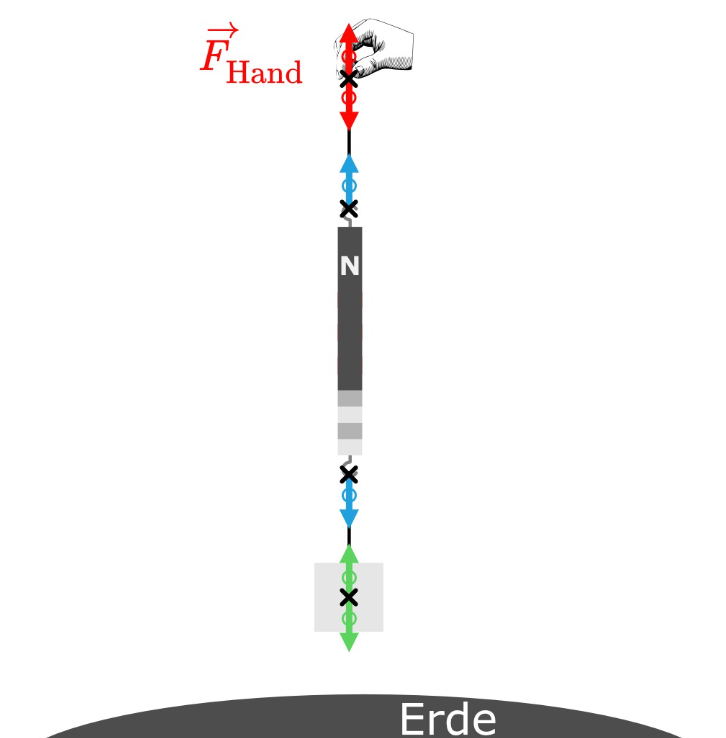
\includegraphics[width=6.3cm]{Bilder/federwaage_kräftegelichgewicht.png}
  \end{minipage}%
  \hfill
  \begin{minipage}[t]{0.48\linewidth}
    \centering
    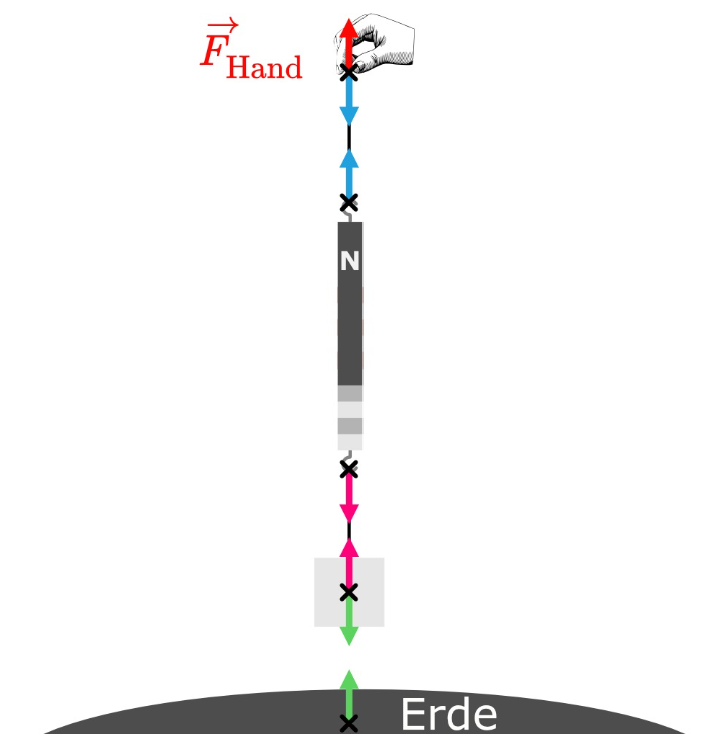
\includegraphics[width=6.3cm]{Bilder/federwaage_Wechselwirkung.png}
  \end{minipage}
\end{center}
\vspace{0.6cm}

Der Grössenunterschied zwischen den beiden Einfärbungen macht den
Unterschied zwischen \glqq an einem Körper\grqq{} und \glqq an zwei
Körpern\grqq{} sichtbar.
\end{solution}
\end{taskbox}

% =============================================================================
% Experiment: Federwaage zwischen zwei 200-g-Massen (LZ3)
% =============================================================================
\needspace{7cm}
\begin{taskbox}[Aufgabe: Federwaage zwischen zwei Massen]
\question[7] Ein Tisch hat auf beiden Seiten je eine Umlenkrolle,
dazwischen ist auf dem Tisch eine Federwaage gespannt. Deren beide Enden
führen über die Rollen zu seitlich hängenden Massen von je
$\SI{200}{\gram}$ ($m_1$ links, $m_2$ rechts):

\Bild{9cm}{Bilder/Federwaage_zwei_massen.jpg}

\begin{parts}
\part[3] \textbf{Variante 1:} Nur $m_1$ ($\SI{200}{\gram}$) hängt auf
einer Seite, die andere Seite ist an einem Stativ fixiert. Welche
Anzeige erwarten Sie (mit $g\approx\SI{10}{\newton\per\kilogram}$,
gerundet für runde Zahlen)?

\Antwortraum{1.5}

\begin{solution}
Die Federwaage befindet sich im Kräftegleichgewicht mit der hängenden
Masse:
\[
F_G = m\cdot g = \SI{0.2}{\kilogram}\cdot\SI{10}{\newton\per\kilogram}
    = \SI{2}{\newton}
\]
Die Anzeige beträgt $\SI{2}{\newton}$.
\end{solution}

\part[4] \textbf{Variante 2:} Statt des Stativs hängt nun auch auf der
zweiten Seite eine Masse, $m_2=\SI{200}{\gram}$ (also
$m_1=m_2=\SI{200}{\gram}$). Vorhersage: Ändert sich die Anzeige?
Beobachtung: Führen Sie den Versuch durch. Erklärung: Begründen Sie über
das Kräftegleichgewicht an jeder Masse einzeln und an der (näherungsweise
masselosen) Federwaage selbst.

\Antwortraum{2.5}

\begin{solution}
Die Anzeige bleibt bei $\SI{2}{\newton}$, obwohl jetzt auf beiden Seiten
je eine Masse hängt statt nur auf einer. An jeder einzelnen Masse hält
die Seilkraft der Gewichtskraft das Gleichgewicht:
\[
F_G = m\cdot g = \SI{0.2}{\kilogram}\cdot\SI{10}{\newton\per\kilogram}
    = \SI{2}{\newton},
\]
das Seil zieht also weiterhin mit $\SI{2}{\newton}$ an jedem Ende der
Federwaage. Auch die (näherungsweise masselose) Federwaage selbst
befindet sich im Kräftegleichgewicht: Weil ihre Masse vernachlässigbar
ist, muss die Nettokraft auf sie null sein (nicht etwa ein
Wechselwirkungspaar, sondern ein Kräftegleichgewicht an ein und
demselben Körper, der Federwaage). Die beiden Zugkräfte an ihren Enden
müssen deshalb exakt gleich gross sein. Das ist hier erfüllt, weil
$m_1=m_2$. Die Federwaage zeigt deshalb in beiden Varianten denselben
Wert, $\SI{2}{\newton}$: Die Zugkraft wird in Variante 1 durch das
Stativ so eingestellt, dass sie der Gewichtskraft von $m_1$ entspricht,
in Variante 2 stellt sich exakt derselbe Wert ein, weil $m_2$ genauso
schwer ist wie $m_1$.
\end{solution}
\end{parts}
\end{taskbox}

% =============================================================================
% Vertiefung: LKW-PKW-Predict + PhysikLibre-Eisflaeche (LZ4, Fortsetzung)
% =============================================================================
\needspace{6cm}
\begin{taskbox}[Aufgabe: Lastwagen und Auto]
\question[4] Ein Lastwagen und ein Auto stossen frontal zusammen:

\Bild{10cm}{Bilder/LKW_vs_PKW.png}

\begin{parts}
\part[2] Vorhersage: Übt der Lastwagen beim Zusammenstoss eine grössere
Kraft auf das Auto aus als das Auto auf den Lastwagen?

\Antwortraum{1}

\part[2] Erklärung: Vergleichen Sie die Kräfte und die Wirkungen auf
beide Fahrzeuge.

\Antwortraum{1.5}

\begin{solution}
Nach dem Wechselwirkungsgesetz sind die Kräfte auf Lastwagen und Auto
exakt gleich gross, die naheliegende Vorhersage aus (a) stimmt also
nicht. Dass sich beim Zusammenstoss scheinbar nur das Auto heftig bewegt,
liegt wie beim Skateboardversuch an der unterschiedlichen Masse: Bei
gleicher Kraft ist die Beschleunigung des leichteren Autos ($a=F/m$)
viel grösser als jene des schweren Lastwagens. Dasselbe Prinzip zeigt
PhysikLibre 4.2.8 am Beispiel zweier Personen auf einer Eisfläche mit
unterschiedlicher Masse.
\end{solution}
\end{parts}
\end{taskbox}

% =============================================================================
% Vertiefung: Magnetwagen als Gedankenexperiment (kein Predict-Observe-
% Explain, da der Wagen nicht real existiert und im Unterricht nicht gezeigt
% werden kann) + Lok auf drehbarem Rad als echtes Predict-Observe-Explain-
% Experiment (LZ5)
% =============================================================================
\needspace{8cm}
\begin{taskbox}[Aufgabe: Magnetwagen]
\question[8] Ein Wagen trägt einen Magneten, der über einen nach vorne
ragenden Arm ein am selben Wagen befestigtes Eisenstück anzieht:

\Bild{8cm}{Bilder/magnetauto.png}

\begin{parts}
\part[3] \textbf{Vorhersage und Begründung:} Fährt der Wagen los, wenn Sie
ihn (reibungsfrei gelagert) loslassen? Begründen Sie Ihre Antwort mit dem
Wechselwirkungsgesetz und dem Begriff \glqq System\grqq.

\Antwortraum{2}

\begin{solution}
Der Wagen bleibt stehen, obwohl Magnet und Eisenstück sich mit einer
Kraft nach dem Wechselwirkungsgesetz gegenseitig anziehen. Beide gehören
aber zum selben System, dem Wagen, weil beide am selben Wagen befestigt
sind. Die beiden Kräfte des Wechselwirkungspaares wirken deshalb beide
auf dasselbe System und heben sich für den Wagen als Ganzes auf. Ein
Fahrzeug kann sich nicht allein durch eine rein interne Kraft selbst
antreiben.
\end{solution}

\part[1] \textbf{Predict:} Gegenüberstellung: Eine Spielzeuglokomotive
fährt auf einer Kreisschiene, die auf einem reibungsfrei drehbar
gelagerten Rad befestigt ist:

\Bild[angle=-90]{7.5cm}{Bilder/lok_auf_rad.jpg}

Was passiert mit der Schiene, wenn die Lokomotive auf ihr losfährt?

\Antwortraum{1}

\part[1] \textbf{Observe:} Führen Sie den Versuch durch (oder beobachten
Sie ihn als Demonstration). Was passiert?

\Antwortraum{1}

\part[3] \textbf{Explain:} Begründen Sie die Beobachtung mit dem
Wechselwirkungsgesetz. Wieso unterscheidet sich dieser Fall vom
Magnetwagen? Und wieso bewegt sich die Schiene dabei sichtbar, obwohl sie
zunächst genauso fest verankert wirken könnte wie die Wand im
Skateboardversuch?

\Antwortraum{1.5}

\begin{solution}
Die Schiene dreht sich zusammen mit dem Rad rückwärts, während die
Lokomotive auf ihr nach vorne fährt. Anders als beim Magnetwagen bilden
Lokomotive und Schiene hier zwei getrennte, je für sich bewegliche
Systeme: Die Lokomotive übt über ihre Räder eine Kraft auf die Schiene
aus, nach dem Wechselwirkungsgesetz wirkt exakt dieselbe Kraft
entgegengesetzt auf die Lokomotive zurück. Weil die Schiene hier
reibungsfrei drehbar gelagert ist, statt (wie die Wand im
Skateboardversuch) über eine riesige effektive Masse zu verfügen,
reagiert sie sichtbar: Sie beschleunigt in die Gegenrichtung.
\end{solution}
\end{parts}
\end{taskbox}

% =============================================================================
% Beispiele: Rueckstossprinzip, Kernbeispiele Rakete und Eisflaeche (LZ6)
% =============================================================================
\needspace{5cm}
\begin{taskbox}[Aufgabe: Rückstossprinzip]
\question[3] Auch beim Start einer Rakete wirkt das Wechselwirkungsgesetz:

\Bild{6.5cm}{Bilder/Rakete.jpg}

Benennen Sie das Wechselwirkungspaar. Auch dies ist ein Beispiel des
Rückstossprinzips.

\Antwortraum{1.5}

\begin{solution}
Die Rakete stösst Treibstoffgase nach hinten aus (Kraft der Rakete auf
die Gase). Nach dem Wechselwirkungsgesetz üben die Gase eine exakt
gleich grosse, entgegengesetzte Kraft auf die Rakete aus, die dadurch
nach vorne beschleunigt wird.
\end{solution}
\end{taskbox}

% =============================================================================
% Abschluss: Partneraufgabe (LZ7)
% =============================================================================
\needspace{7cm}
\begin{taskbox}[Aufgabe: Eigene Alltagssituation]
\question[5] Skizzieren Sie selbständig eine eigene Alltagssituation
(nicht eines der heute bereits behandelten Beispiele) mit mindestens
einem eindeutigen Wechselwirkungspaar.

\begin{parts}
\part[2] Ihre eigene Skizze:

\Antwortraum{2}

\part[3] Einzelne Skizzen werden anschliessend im Plenum vorgestellt.
Zeichnen Sie gemeinsam die dort wirkenden Kräfte ein und markieren Sie
zusätzlich, wo (falls vorhanden) ein Kräftegleichgewicht vorliegt. Prüfen
Sie dabei: Sind an jedem Körper alle wirkenden Kräfte im Gleichgewicht
vollständig erfasst? Sind Wechselwirkungspaare als je zwei Pfeile an zwei
verschiedenen Körpern mit gleicher Länge, Gegenrichtung und gleicher
Wirkungslinie dargestellt?

\Antwortraum{2.5}
\end{parts}
\end{taskbox}
\end{questions}

Weitere Übungsaufgaben zur Wechselwirkung finden Sie im separaten
Aufgabenblatt.

\end{document}
